%*****************************************
\chapter{Beispiele}\label{ch:examples}
%*****************************************

% Beispiele f�r die folgenden Themenbereiche noch einfügen
% \begin{itemize}
% 	\item biblatex (zusammen mit JabRef)
% 	%\item jpeg foto
% 	%\item pdf diagramm + visio vorlage (liefert AM) + jpg falsch
% 	%\item png screenshot
% 	%\item Quellcode aus Datei + aus Snippet (mit Highlighting)
% 	%\item Abb./Sektionen etc. referenzieren
% 	%\item todonotes für Anmerkungen
% 	%\item Tabellen
% 	%\item Abbildungen mit mehreren Bildern
% 	%\item Abkürzungen
% 	%\item Formeln
% 	\item Verweise auf Quellen (siehe biblatex oben)
% 	\item htw saarlogo als pdf noch für Titelblatt
% 	\item PDF-Booksmarks für Table of Contents etc. einfügen (gibt KOMA-Option dafür)
% \end{itemize}

%************************************************
%*  Abk�rzungen *********************************
%************************************************

\section{Abk�rzungen}

Um Abk�rzungen zu verwenden, muss �ber \lstinline|\usepackage{acronym}| das ben�tigte Package geladen werden.

Ein kleiner Test k�nnte so aussehen: \\

Dies ist eine \ac{Abk.}, die beim ersten Aufruf mit Erkl�rung und bei allen weiteren Malen nur als \ac{Abk.} dargestellt wird. Auch der Plural von \aclp{Abk.} kann definiert und abgerufen werden. Mit anderen Befehlen kann man auch die Erkl�rung mitliefern \acf{z.B.} so. Wer nur die Abk�rzung mag, f�gt sie \acs{z.B.} so ein. Mit \lstinline|\acused{Abk.}| wird die \acl{Abk.} als genutzt markiert und taucht im Folgenden nur noch in seiner Kurzform auf.
 
 Ganz am Ende der Arbeit wird das Abk�rzungsverzeichnis eingef�hrt (auch als eigenes Chapter m�glich): 

\begin{acronym}
 	\acro{Abk.}{Abk�rzung}
 	\acroplural{Abk.}[Abk.]{Abk�rzungen}
 	\acro{z.B.}{zum Beispiel}
\end{acronym}

Weitere Informationen sind im \textit{Acronym-Manual} zu finden.
%*********************************************
%*	Biblatex-Beispiel
%*********************************************
\section{Beispiel f�r BibLaTeX}

BibLaTeX ist ein Package, das einem die Arbeit mit Zitaten bzw. Quellenangaben erleichtern kann. Mit JabRef (\autoref{sec:Werkzeuge}) ist es m�glich
\textit{*.bib}-Dateien zu erstellen, in denen alle Angaben zu Autor, Buchtitel, Erscheinungsdatum usw. hinterlegt werden, welche zum passenden Zeitpunkt
abgerufen werden k�nnen. Das Literaturverzeichnis wird mittels \lstinline{\printbibliography} ausgegeben.

Im Allgemeinen wird im Literaturverzeichnis auch nur jene Literatur aufgenommen, die auch in der \textit{*.tex}-Datei referenziert wird. Danach ist es wichtig
nicht nur mit \textit{Pdf\-LaTeX}, sondern auch mit \textit{BibLaTeX} zu kompilieren, damit die zitierten Eintr�ge in die verschiedenen Hilfsdateien aufgenommen
werden k�nnen. %Hinweis: Pdf\-LaTeX teilt LaTeX mit, dass nur zwischen Pdf und LaTeX getrennt werden darf


\subsection{Einige Zitate}
In diesem Satz k�nnten wir auf \cite{knuth:1976} verweisen, ebenso auf das wichtige Werk \cite{dueck:trio}. Wenn uns das nicht genug ist, sollten wir das anmerken,
was in \cite{sommerville:1992} geschrieben wurde. Im Zweifelsfall verweisen wir auf eine einzelne Seite, wie in \cite[112]{bentley:1999} zu finden. 

�blicherweise wird auch der Name des Autors bzw. der Autoren genannt, also beispielsweise bei einem Verweis auf \citeauthor{knuth:1976} \cite{knuth:1976} oder 
auch bei mehreren Autoren \citeauthor{cormen:2001} \cite{cormen:2001}. LaTeX stellt Mechanismen zur Verf�gung, auch dies automatisiert zu erledigen.





\section{Referenzierungen}
Mit Referenzierungen kann ich ganz bequem auf Textpassagen, Kapitel, Sections oder Abbildungen im weiteren Text verweisen.
Dies ist ein Verweis auf Unterabschnitt \ref{subsec:Beispieltext}, die sich auf Seite \pageref{subsec:Beispieltext} befindet.

Auch ein Verweis auf Tabelle \ref{tab:beispieltabelle1} auf Seite \pageref{tab:beispieltabelle1} ist m�glich.

Man sollte beachten, dass man sein Dokument, wenn es Referenzierungen enth�lt, mehrmals kompiliert, da sonst manche
Verweise nicht aufgel�st werden k�nnen.


\subsection{Beispieltext}
\label{subsec:Beispieltext}
\blindtext
\blindtext
\blindtext
\section{Dateien einbinden}

Damit man nicht alle Einstellungen, Optionen, Packages und Texte, Abbildungen etc. in einer Datei unterbringen muss, werden
zwei Befehle bereitgestellt, um externe \textit{*.tex}-Dateien einzubinden: \lstinline|\include{PFAD}| und \lstinline|\input{PFAD}|.
Mit dem erstem Befehl wird eine neue Seite angelegt, danach kommen die Inhalte aus der angegebenen Datei; mit dem zweiten
Befehl wird keine neue Seite angelegt -- der Inhalt der angegebenen Datei wird direkt an die betroffene Stelle eingef�gt.

\textbf{Wichtig:} Der \textit{Pfad} wird sinnigerweise \textit{relativ} angegeben, wobei als Stammverzeichnis jenes Verzeichnis
angesehen wird, in dem die \textit{*.tex}-Datei mit der \textit{Document}-Umgebung abgelegt ist (in diesem Fall ist es 
\textit{htwsaar-i-mst-config.tex}).
%************************
%*		Tabellen 		*
%************************

\chapter{Tabellen}

\section{Einfache Tabelle}
In LaTeX lassen sich Tabellen unterschiedlicher Ausprägung einfach erzeugen. Das allgemeine Format einer Tabelle sieht aus wie folgt:

\begin{lstlisting}[caption={Allgemeines Format}]
\begin{table}
	\caption{BESCHRIFTUNG}
	\begin{tabular}{FORMATIERUNG}
		TABELLENINHALT
	\end{tabular}
\end{table}
\end{lstlisting}

Eine Beispieltabelle (Tabelle \ref{tab:beispieltabelle1}) könnte also so aussehen:

\begin{lstlisting}[caption={Tabelle \ref{tab:beispieltabelle1}}]
\begin{table}
	\caption{Beispiel 1}
	\begin{tabular}{l|r|c|r}
		\toprule
		\textbf{Name} & \textbf{Vorname} & \textbf{Matrikelnummer} & \textbf{Lieblingsspeise}\\
		\midrule
		Jackson & Michael & 123456 & Erdbeereis \\
		Springsteen & Bruce & 234567 & Schwedisches Lakritz \\
		Bach & Anna, Magdalena & 3456789 & Frankfurter Kranz \\
		Schumann & Clara & 4567890 & Bisquittörtchen \\
		\bottomrule
	\end{tabular}
	\label{tab:beispieltabelle1}
\end{table}
\end{lstlisting}

Mit \lstinline|\caption{Beispiel 1}| bekommt unsere Tabelle eine Beschriftung am Tabellenkopf. \lstinline{l|r|c|r} legt die Textausrichtung der einzelnen Spalten fest: \lstinline|l| bedeutet linksausgerichtet, \lstinline|r| rechtsausgerichtet und \lstinline|c| zentriert. Durch \lstinline{|} werden Spaltenlinien gezogen. \lstinline|\toprule|, \lstinline|\midrule| und \lstinline|\bottomrule| erzeugen Kopf-, Mittel- und Abschlusslinie in der Tabelle. Als Spaltentrenner wird das \lstinline{&} genutzt, Zeilentrenner ist der doppelte Backslash (\lstinline|\\|). Am Ende kann die Tabelle auch mit einem Label versehen werden (\lstinline|\label{tab:beispieltabelle1}|), über welches diese referenziert wird.

%\begin{center}
\begin{table}[b]
	
	\caption{Beispiel 1}
	\begin{tabular}{l|r|c|r}
		\toprule
		\textbf{Name} & \textbf{Vorname} & \textbf{Matrikelnummer} & \textbf{Lieblingsspeise}\\
		\midrule
		Jackson & Michael & 123456 & Erdbeereis \\
		Springsteen & Bruce & 234567 & Schwedisches Lakritz \\
		Bach & Anna, Magdalena & 3456789 & Frankfurter Kranz \\
		Schumann & Clara & 4567890 & Bisquittörtchen \\
		\bottomrule
	\end{tabular}
	\label{tab:beispieltabelle1}
\end{table}
%\end{center}

\section{Erweiterte Tabellenbefehle}
Um Tabellen in LaTeX flexibler zu gestalten gibt es weitere Befehle bzw. zusätzliche Pakete, die einem das Leben leichter machen (Tabelle \ref{tab:beispieltabelle2}). Hierzu ein weiteres Beispiel:

\begin{lstlisting}[caption={Tabelle \ref{tab:beispieltabelle2}}]
\begin{table}
	\centering
	\caption{Beispiel 2}
	\begin{tabular}{|l|l|l|}
		\hline
		Author & Title & Year \\
		\hline
		\hline
		\multirow{3}{*}{Stanislav Lem} & Solaris & 1961 \\
 			& Robotermärchen & 1967 \\
 			& Der futurologische Kongress & 1971 \\
		\hline
		\multirow{3}{*}{Isaac Asimov} & Ich, der Robot & 1952 \\
 			& Der Tausendjahresplan & 1966 \\
 			& Doctor Schapirows Gehirn & 1988 \\
		\hline
	\end{tabular}
\label{tab:beispieltabelle2}
\end{table}
\end{lstlisting}

Mit \lstinline|\centering| wird die Tabelle zentriert ausgerichtet, analoge Befehle für rechts- bzw. linksausrichtung sind z.B. \lstinline|\raggedleft| und \lstinline|\raggedright|. \\

Eine weitere Form der Tabellen ist das package \textit{tabularx}, das variable Spaltenbreiten unterstützt, und \textit{booktabs}, welches mit horizontalen Linien besser arbeiten kann.
\begin{table}
	\centering
	\caption{Beispiel 2}
	\begin{tabular}{|l|l|l|}
		\hline
		Author & Title & Year \\
		\hline
		\hline
		\multirow{3}{*}{Stanislav Lem} & Solaris & 1961 \\
 			& Robotermärchen & 1967 \\
 			& Der futurologische Kongress & 1971 \\
		\hline
		\multirow{3}{*}{Isaac Asimov} & Ich, der Robot & 1952 \\
 			& Der Tausendjahresplan & 1966 \\
 			& Doctor Schapirows Gehirn & 1988 \\
		\hline
	\end{tabular}
\label{tab:beispieltabelle2}
\end{table}
\section{Abbildungen}
%=============================

\textit{LaTeX} unterst�tzt generell die Formate \textit{*.jpeg}, \textit{*.png} und \textit{*.pdf}.
Handelt es sich z.B. um Strichgrafiken oder skalierbare Farbfl�chen, sollte \textit{*.pdf} die erste Wahl sein,
da dieses Format sich ohne Qualit�tsverlust skalieren l�sst.

\subsection{Eine erste Abbildung}

\blindtext
\begin{figure}[htbp] 
  \centering
  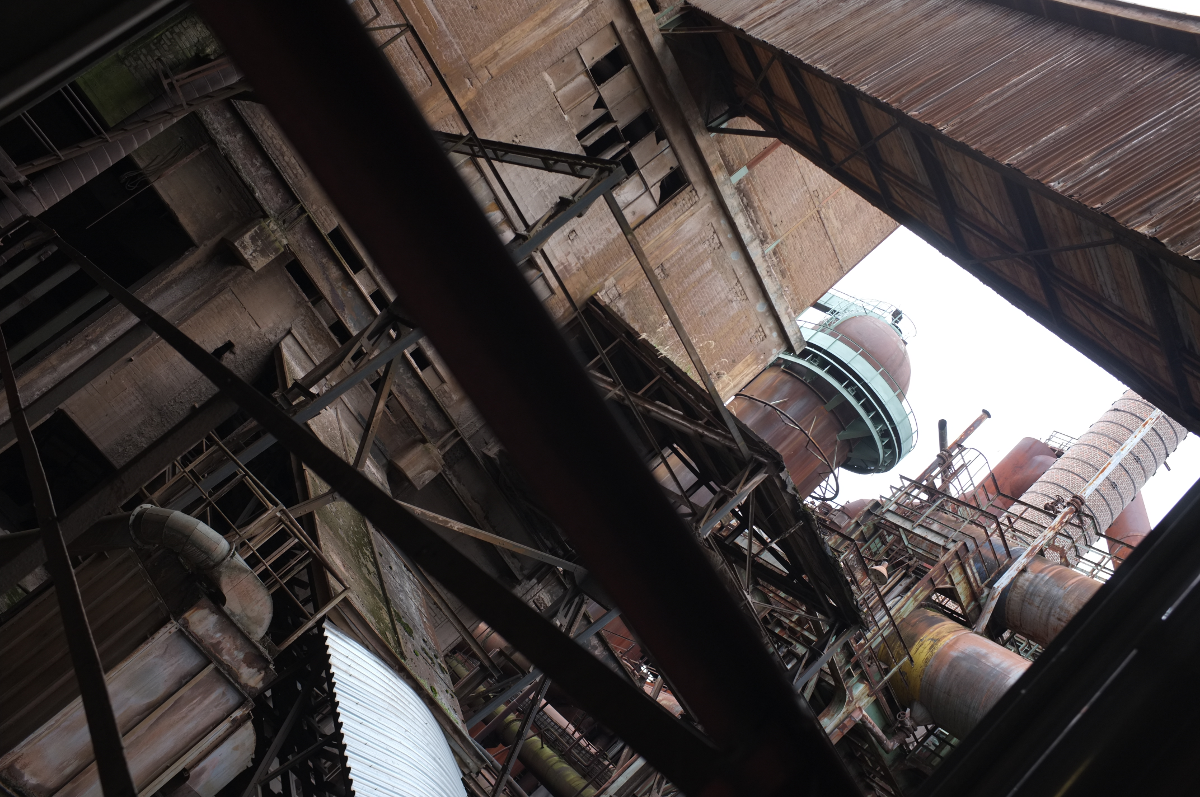
\includegraphics[width=0.7\textwidth]{Examples/example_5.png}
  \caption{Erstes Bild, V�lklinger H�tte}
  \label{fig:Huette}
\end{figure}

\subsection{Es geht besser}

Abbildung \ref{fig:Huette} ist zwar ganz nett anzusehen, aber vielleicht s�he es eleganter aus, wenn die Abbildung 
von unserem Textabschnitt umflossen wird.


\blindtext
\begin{wrapfigure}{l}{0.5\textwidth}
  \centering
  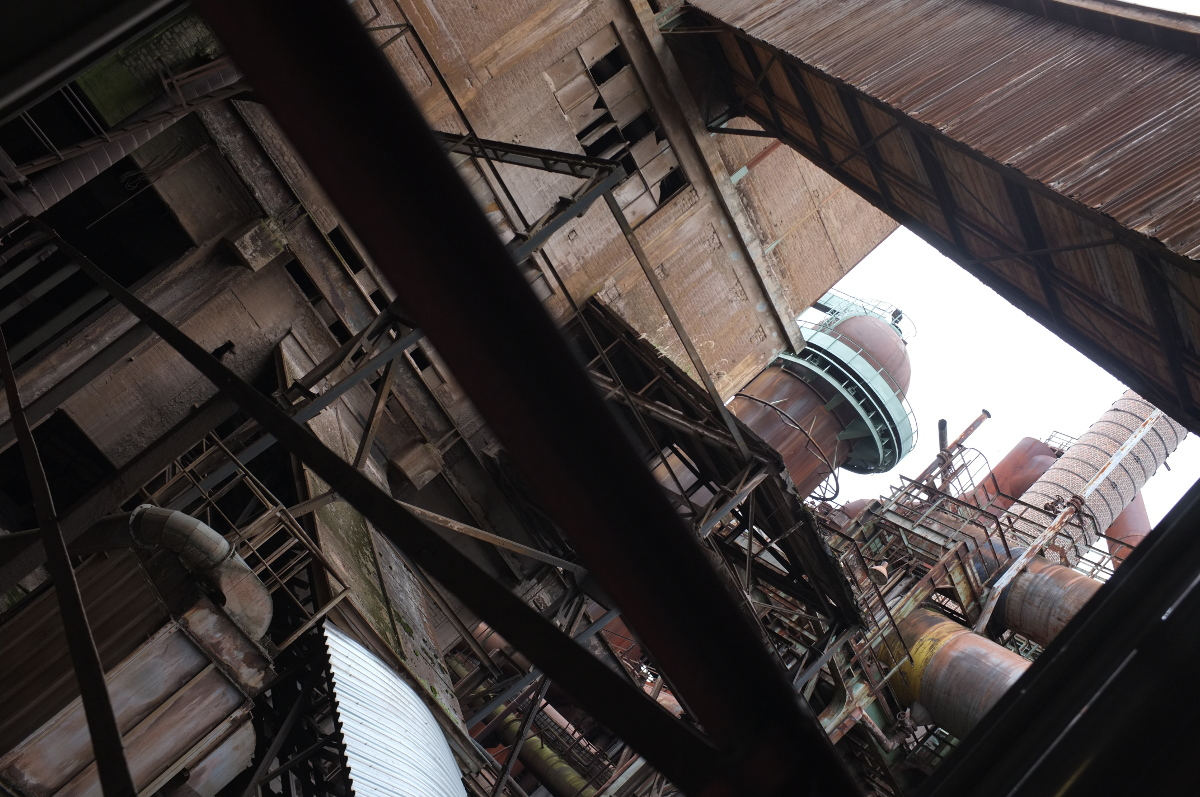
\includegraphics[width=0.5\textwidth]{Examples/example_5.jpg}
  \caption{V�lklinger H�tte, *.jpg}
  \label{fig:Huette2}
\end{wrapfigure}
\blindtext
\blindtext

\subsection{Mehrere Abbildungen nebeneinander}

Es ist ebenso m�glich mehrere Abbildungen nebeneinander zu setzen, wie in Abbildung \ref{fig:Beide} zu sehen ist.

\begin{figure}
  \subfloat[Erstes ...]{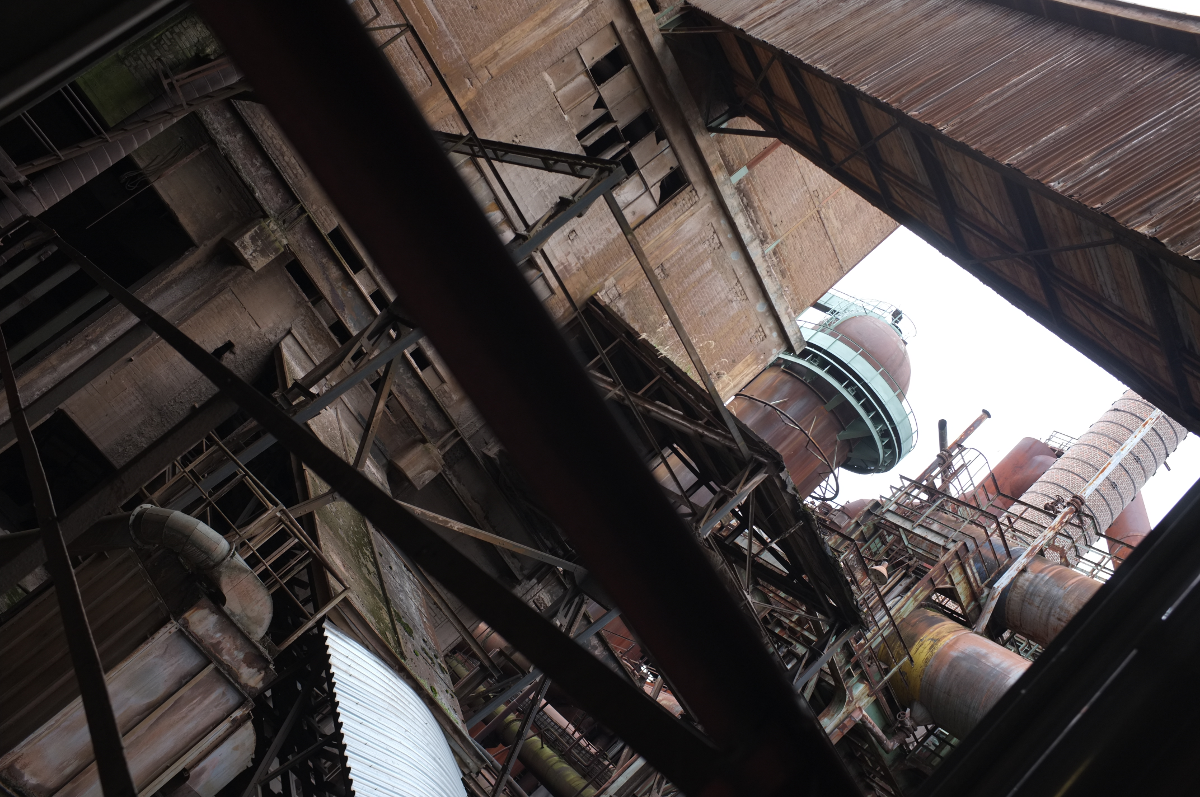
\includegraphics[width=0.49\textwidth]{Examples/example_5.png}}\hfill
  \subfloat[... und zweites Bild]{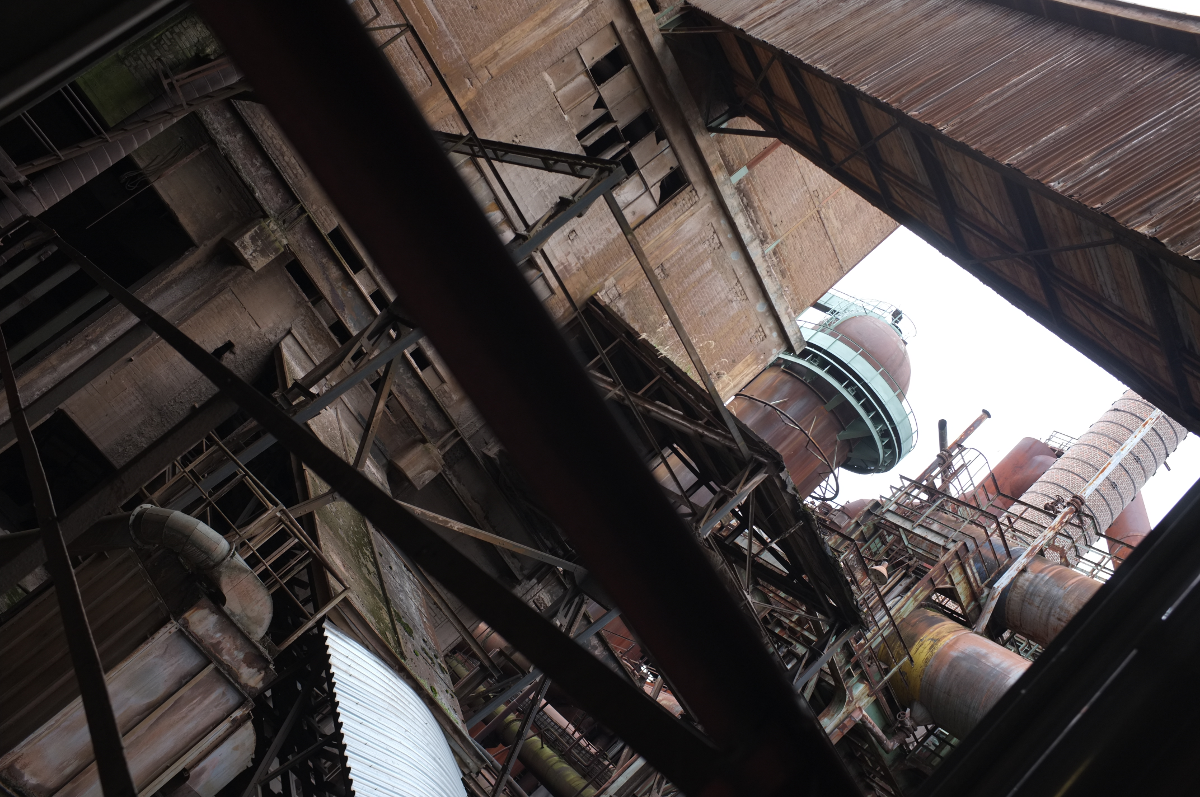
\includegraphics[width=0.49\textwidth]{Examples/example_5.png}}
  \caption{Abbildung \ref{fig:Huette} und \ref{fig:Huette2} nebeneinander}
  \label{fig:Beide}
\end{figure}

\subsection{Qualit�tsunterschiede}

\begin{figure}[p]
	\centering
  \subfloat[\textit{PDF}-Format]{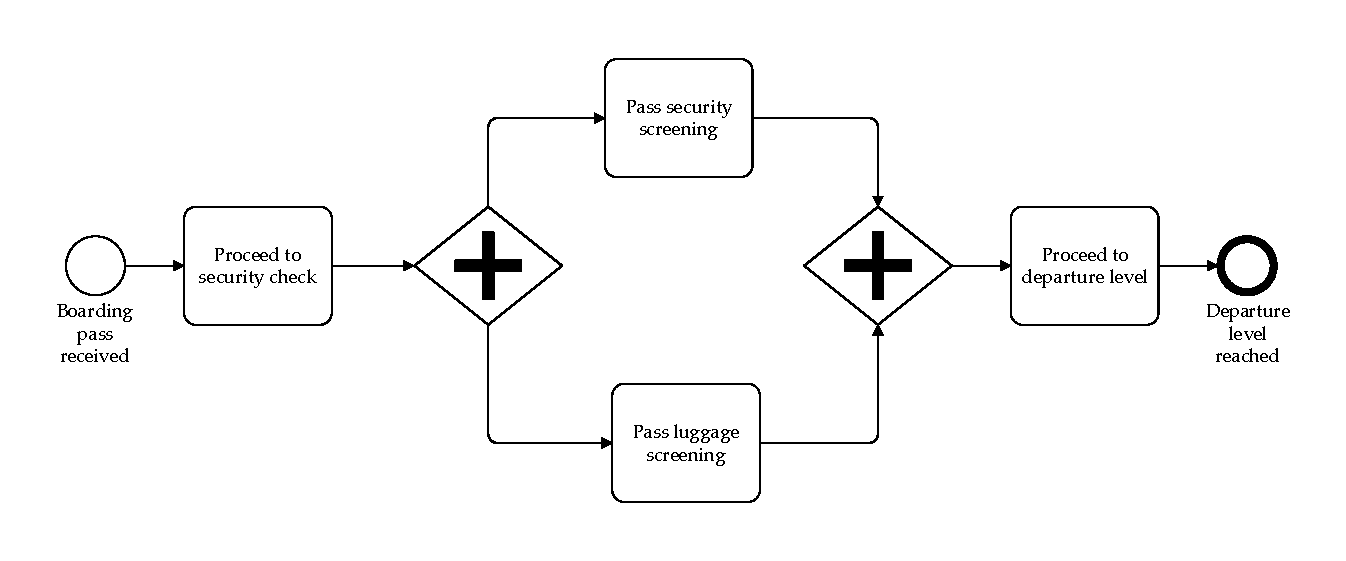
\includegraphics[width=0.65\textwidth]{Examples/bpmn.pdf}} \\
  \subfloat[\textit{JPG}-Format]{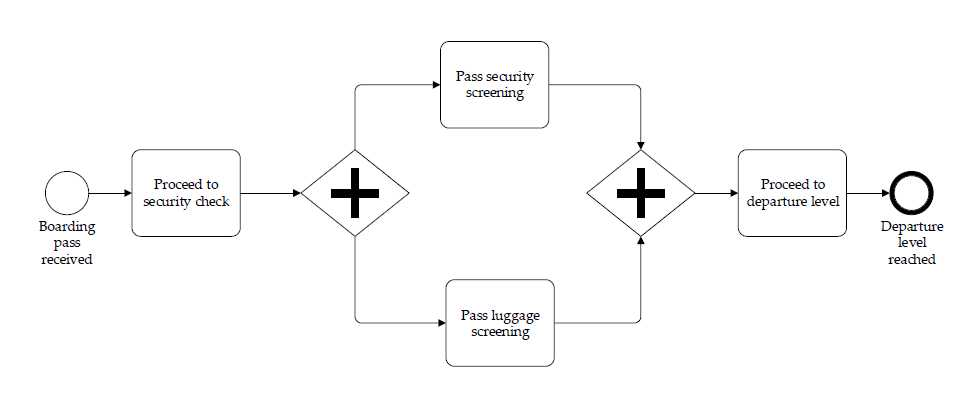
\includegraphics[width=0.65\textwidth]{Examples/bpmn.jpg}}
  \caption{Beide Formate im Vergleich}
  \label{fig:pdfvsjpg}
\end{figure}

\begin{figure}[p]
	\centering
  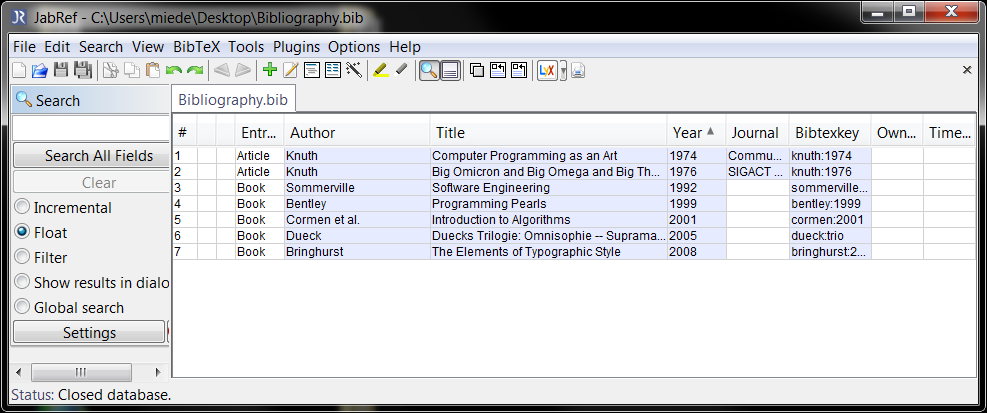
\includegraphics[width=0.65\textwidth]{Examples/jabref.PNG}
   \caption{\textit{PNG}-Format}
  \label{fig:pngvsjpg1}
\end{figure}

\begin{figure}[p]
	\centering
  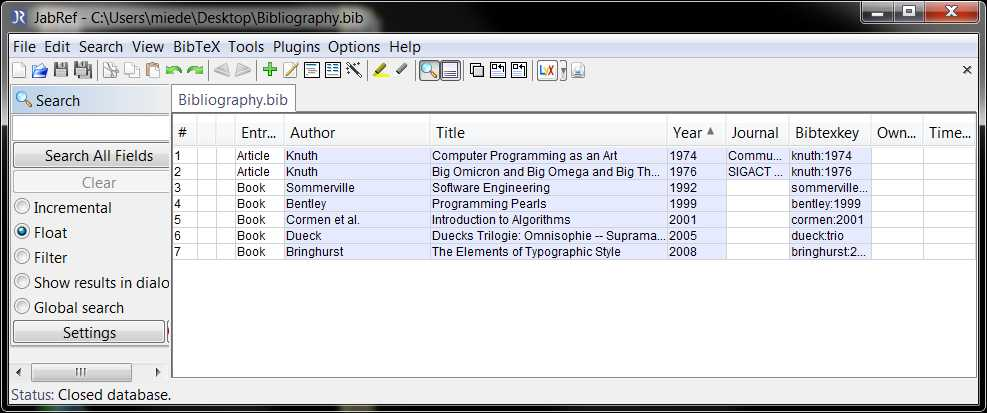
\includegraphics[width=0.65\textwidth]{Examples/jabref.jpg}
   \caption{\textit{JPG}-Format}
  \label{fig:pngvsjpg2}
\end{figure}

Leider haben die unterschiedlichen Grafikformate bedingt durch die unterschiedlichen Kompressionsverfahren einige Schw�chen, insbesondere
die Umwandlung in das \textit{JPG}-Format erzeugt unangenehme Artefakte im Bild. \autoref{fig:pdfvsjpg} zeigt die Unterschiede zwischen
\textit{PDF-Format} und \textit{JPG-Format} im Vergleich. 

Wenn eine \textit{*.pdf}-Datei nicht infrage kommt, beispielsweise bei Screenshots, ist unbedingt das \textit{PNG-Format} vorzuziehen. 
Den Unterschied machen \autoref{fig:pngvsjpg1} und \autoref{fig:pngvsjpg2} deutlich.


\glqq Faustregeln\grqq im Umgang mit Abbildungen:
\begin{itemize}
	\item Diagramme bzw. alles, was Linien usw. enth�lt: \textit{PDF}.
	\item Screenshots bzw. alles, was gr��ere gleichfarbige Fl�chen enth�lt: \textit{PNG}.
	\item Der Rest (in der Regel Fotos): \textit{JPEG}.
\end{itemize}





%*******************************
% 			Listings 		   *
%*******************************

\section{Quellcode einbinden}
Das Package \textit{lstlisting} erm�glicht es, Quellcode ansprechend in das Dokument einzubinden. Man kann Quellcode einzeilig einbinden 
mittels \lstinline{\lstinline|Quellcode|}. Dabei ist darauf zu achten, dass der Befehl einmal mit \{ \} und einmal mit | | aufgerufen werden kann, je nachdem, 
welche Zeichen im angegebenen Quelltext genutzt werden. 
Es ist auch m�glich eine eigene Umgebung f�r Quelltext zu schaffen:

\begin{lstlisting}[caption=Erstes Listing,style=Java]
private Umgebung(int i, int k)
{
	System.out.println("Eine Funktion mit " + i + "und" + k ".");
}
\end{lstlisting}  

Wer Quelltext aus externen Dateien einbinden m�chte, geht wie folgt vor:

\lstinputlisting
[caption={Externer Quellcode},style=Java]
{Examples/Code.java}

Wie genau der Quellcode formatiert und gef�rbt ist, ist in \textit{htwsaar.i.mst.config.tex} hinterlegt, wobei f� verschiedene Sprachen auch eigene Styles angelegt werden
k�nnen (hier z.B. f�r Java).
\chapter{Mathematische Ausdrücke}
\section{Allgemeines}
%********************************************

Mathematische Ausdrücke sind eine kleine Kunst für sich. Am allereinfachsten kann man eine Formel, wie \(a + b = c\) in den Fliesstext einbinden, wobei Latex die Höhe der Ausdrücke der Zeile an passt, wie hier zu sehen \(\sum_{y=0}^{x} a\) . In einer Umgebung sieht das schon anders aus:

\begin{equation}
  \sum_{y=0}^{x} a
\end{equation}

\section{Mathematisches}
\subsection{Brüche}
%********************************************

\begin{equation}
Ergebnis = \frac{a}{b}
\end{equation}

\begin{equation}
\frac{\sin{\alpha}^2 + \cos{\alpha}^2}{1} = 1
\end{equation}

\begin{equation}
\frac{-9x}{\frac{2y}{3z+2}}
\end{equation}

\subsection{Hoch- bzw. Tiefstellungen}
%********************************************

\begin{equation}
x_{i,j}^2
\end{equation}

\begin{equation}
{x_{i,j}}^2
\end{equation}

\begin{equation}
x_{n_0}
\end{equation}

\subsection{Text innerhalb von Formeln}
%********************************************

\begin{equation}
\sum_{y=1}^{n} y = \frac{n*(n+1)}{2}
\quad
\text{Gaus'sche Summenformel}
\end{equation}

\subsection{Matrizen}
%********************************************

Matrizen werden innerhalb der mathematischen Umgebung als wiederum neue Umgebung eingebunden. Wie bei Tabellen auch werden Zeilen durch \lstinline{\\} und Spalten durch \lstinline{&} getrennt.

\begin{equation}
\begin{pmatrix} 
a&b\\
c&d 
\end{pmatrix}
\end{equation} 

\begin{equation}
\begin{vmatrix} 
a&b\\
c&d 
\end{vmatrix}
\end{equation} 

\subsection{Fallunterscheidung}
%********************************************

\begin{equation}
f(x) = 
\begin{cases}
0, &\text{falls } x < 0 \\
1, &\text{falls } x \geq 0
\end{cases}
\end{equation}

\subsection{Ein paar griechische Buchstaben}
%********************************************

\begin{equation}
\alpha\beta\gamma\delta\epsilon\varepsilon\zeta\eta
\theta\iota\kappa\lambda\mu\nu\xi\pi\varpi\rho\varrho
\sigma\tau\upsilon\phi\varphi\chi\psi\omega
\end{equation}


% Eigene Shortcuts fuer laengere Befehle
\newcommand{\todox}[1]{\todo[inline, size=\small]{#1}}

%Nummerierte Anmerkungen
\newcounter{todocounter}

\renewcommand{\todox}[2][]{\stepcounter{todocounter}\todo[inline, size=\small,caption={\thetodocounter: #2}, #1]{\renewcommand{\baselinestretch}{0.5}\selectfont\thetodocounter: #2\par}}

%############################################################

\section{To-Do-Notes}

Um bei einer l�ngeren Arbeit nicht den �berblick zu verlieren, an welcher Stelle es n�tig ist
weiter zu arbeiten, bietet es sich an kleine Notizen einzuf�gen. Das Latexpackage \textit{todonotes}
stellt eine elegante L�sung bereit, um differenziert und vielfarbig jene Abschnitte zu kennzeichnen,
die einer weiteren Bearbeitung bed�rfen.

\subsection{Beispiel f�r To-Do-Notes}


Lorem ipsum dolor sit amet, consectetuer adipiscing elit. Nulla
\todo{Plain todonotes.}%
urna. Maecenas interdum nunc in augue. Mauris quis massa in ante
tincidunt mollis. Proin imperdiet. Donec porttitor pede id est. Sed
in ante. Integer id arcu. Nam lectus nisl, posuere sit amet,
imperdiet ut, tristique ac, lorem. In erat. In commodo enim.
\todo[color=blue!40]{Todonote with a different color.}%
Phasellus libero ipsum, tempor a, pharetra consequat, pellentesque
sit amet, sem. Praesent ut augue luctus elit adipiscing ultricies.
Vestibulum suscipit cursus leo. Nullam molestie justo.


Morbi dui. Morbi convallis mi sed sem. Nulla convallis lacus vitae
risus. Phasellus adipiscing. Nullam tortor. Sed laoreet aliquam
ante. Vestibulum diam. Pellentesque nec leo. Pellentesque velit.
\todo[nolist]{Todonote that is only shown in the margin and not in
the list of todos.}%
Praesent congue mi eu ipsum cursus fringilla. Etiam leo erat,
tristique et, pharetra eget, mollis vitae, velit. In hac habitasse
\todo[size=\small, color=green!40]{A note with a small fontsize.}%
platea dictumst. In quam nibh, facilisis et, laoreet non, facilisis
tempus, justo.

\todo[inline]{A very long todonote that certainly will fill more
than a single line in the list of todos. Just to make sure let's add
some more text \ldots}

Donec nulla lectus, faucibus sit amet, auctor non, consectetuer
quis, pede. Nullam dictum. Nullam suscipit, ligula in scelerisque
\todo[noline]{A note with no line back to the text.}%
posuere, sapien purus rutrum magna, vitae pharetra leo quam vel
tortor. Donec eleifend condimentum sapien. Etiam sed orci. Aliquam
\todo[inline, color=red!50]{Inline todonotes.}%
tempor. Pellentesque egestas tortor id eros. Donec mauris justo,
commodo id, pellentesque id, eleifend non, mi. Duis venenatis
\todo[caption={A short entry in the list of todos}]{A very long
todonote that certainly will fill more than a single line in the
list of todos \ldots}
sagittis metus. 

\clearpage

\missingfigure{A figure I have to make \ldots}

%Nummerierte ToDo-Notes
\todox{Erste Nummer...}

\missingfigure[figwidth=\textwidth]{A figure I have to make \ldots}

\todox{Zweite Nummer...}

\clearpage

%Alles To-Do's als Liste ausgegeben
\listoftodos


